\section{Experiment}
We first introduce the detailed experimental setup and then present the main results on several NLU tasks followed by a visualization case study.
\subsection{Experiment Setup}
\textbf{Visual Grounding.}~~We use MS COCO~\citep{mscoco} as the multimodal dataset $D_{train}$ for visual grounding. After preprocessing, we get 414,113 image-sentence pairs in the training set and 202,654 pairs in the validation set. Sentences longer than 20 tokens are truncated. Other multimodal resources like Flickr30k ~\citep{flickr} can also be leveraged in the future.

We use pretrained BERT-base-uncased~\citep{devlin-etal-2019-bert} as the text encoder, which contains 12 transformer layers, each having 12 attention heads with hidden size 768. We set the number of adapter blocks $M$ as 3 and place them at 1/6/12-th transformer block in BERT. Each adapter block has $N=2$ transformer layers with hidden size 128. We use AdamW~\citep{adamw} optimizer with an initial learning rate of 3e-4 and batch size of 16.

\textbf{Finetuning.}~~We evaluate the effectiveness of AVG on five multiple-choice question answering tasks: CommonsenseQA~\citep{csqa}, SocialIQA~\citep{socialiqa}, PIQA~\citep{piqa}, CosmosQA~\citep{cosmosqa}, and OpenbookQA~\citep{openbookqa}, as well as 3 classification tasks in GLUE~\citep{glue}: RTE, SST-2, and MRPC.

\textbf{Baselines.}~~We denote AVG with BERT text encoder as BERT-AVG and compare it with the following models: vanilla BERT, BERT-Voken~\citep{voken}, BERT-MACD~\citep{macd}, OSCAR~\citep{oscar}, and BERT-AVG$_r$ with a randomly initialized adapter.
\begin{table}[t!]
	\centering
	\small
	\begin{tabular}{l|ccc}
		\toprule
		\textbf{Model} & Parameters & Time~(h) & Corpus  \\
		\midrule
		BERT-Voken & 110M & 96   & Wikipedia \\
		BERT-MACD & 138M & 15   & COCO\\
		OSCAR & 111M &  - & Misc.\\
		\midrule
		BERT-AVG & 17M & 4 & COCO\\
		\bottomrule
	\end{tabular}
	\caption{Pretraining statistics of VLP methds. Misc includes COCO, Flickr30k, SBU Caption~\citep{sbu}, Conceptual Caption~\citep{cc} and GQA~\citep{gqa}.}
	\label{table:stats}
\end{table}
\begin{table*}[t!]
	\centering
	\footnotesize
	\begin{tabular}{l|ccc|ccccc}
		\toprule
		\multirow{2}{*}{\textbf{Model}} & \multicolumn{3}{c|}{\textbf{Visual heavy tasks}} & \multicolumn{5}{c}{\textbf{NLP heavy tasks}}
		 \\
		&CommonsenseQA &PIQA &OpenbookQA &SocialIQA &CosmosQA &RTE &SST-2 &MRPC \\
		\midrule
		BERT &58.0 &64.9 &56.4 &62.7 &61.9 &70.8 &92.6 &87.0 \\
		BERT-Voken &47.4 &61.8 &51.3 &59.1 &57.4 &61.0 &89.6 &83.6 \\
		BERT-MACD &58.3 &66.9 &55.8 &62.7 &61.6 &68.2 &92.6 &83.2 \\
		OSCAR &48.0 &64.7 &52.8 &54.7 &47.8 &56.0 &89.2 &71.1 \\
		\midrule
		BERT-AVG$_r$ &58.3 &67.5 &57.4 &62.7 &61.8 &70.3 &92.5 &87.3 \\
		BERT-AVG &\textbf{59.1} &\textbf{68.6} &\textbf{58.5} &62.7 &61.8 &\textbf{71.3} &92.9 &87.3 \\
		\bottomrule
	\end{tabular}
	\caption{Downstream performance on pure-text understanding tasks. Best results with statistical significance~(measured by paired student's t-test) are bolded.}
	\label{table:main}
\end{table*}
\subsection{Main Results}
\label{sec:main}
\textbf{Pretraining Efficiency.}



As shown in \tabref{table:stats}, AVG has substantially fewer trainable parameters 
compared to other VLP methods, making it more efficient to train with limited 
computing resources. Total pretraining time for each model is tested on 
a single RTX 2080Ti with 12GB memory.

\textbf{Downstream Performance.}~~We report the best development set performance averaged from 5 runs with different random seeds.


\tabref{table:main} shows the full results of all models. OSCAR is the only model that uses a joint encoder during pretraining~(top left in \figref{fig:intro}) and performs worst among all compared VLP models. It indicates that vision-language pretraining solely on visually-grounded corpus suffer from degraded pure-text modeling capability. BERT-Voken~(top right in \figref{fig:intro}) performs worse than BERT because it only utilizes Wikipedia for pretraining while BERT also includes BookCorpus~\citep{bookcorpus}. Unsurprisingly, BERT-MACD~(bottom left in \figref{fig:intro}) outperforms BERT in CommonsenseQA and PIQA, which largely hinges on perceptual knowledge in the external world. However, it shows significant drops on other vision-insensitive tasks. It is worth noting that BERT-AVG$_r$ already stably surpass all baselines, which is likely due to the additionally introduced parameters in adapter. BERT-AVG brings further improvement on 4 tasks that can benefit from grounded inference. It is also comparable or marginally outperforming BERT on the remaining NLP heavy tasks. It demonstrates the structural flexibility of adapter for leveraging multimodal knowledge of which the usefulness on specific tasks is unknown.
\begin{table}[t!]
	\centering
	\small
	\begin{tabular}{l|ccc}
		\toprule
		\textbf{Model} & CSQA. & PIQA  &OpenbookQA   \\
		\midrule
		RoBERTa &58.5  &65.3 &57.2   \\
		RoBERTa-AVG$_r$ &59.0 &67.0  &57.3  \\
		RoBERTa-AVG &\textbf{60.0}  &\textbf{69.1} &\textbf{59.3} \\
		\midrule
		MPNet &66.9  & 65.4  &58.5  \\
		MPNet-AVG$_r$ &67.9  &69.4  &58.6 \\
		MPNet-AVG &\textbf{68.8}  &\textbf{70.6}  &\textbf{59.8} \\
		\bottomrule
	\end{tabular}
	\caption{Results of AVG upon RoBERTa and MPNet.}
	\label{table:rm}
\end{table}

We also show the transferability of AVG to RoBERTa~\citep{DBLP:journals/corr/abs-1907-11692} and MPNet~\citep{mpnet} in \tabref{table:rm}. We observe similar improvement on visual heavy tasks as in BERT.

\subsection{Case Study}
To glean insight on how AVG helps language understanding, we perform a case study using Integrated Gradient~\citep{ig}, a gradient-based attribution method for interpreting model decisions. We show one instance from the development set of PIQA, on which both BERT and BERT-AVG$_r$ failed but BERT-AVG correctly answered.

\figref{fig:IG} displays the feature saliency map with respect to the input embedding of each token. It can be observed that while both BERT and BERT-AVG$_r$ fail to compose ``apple'' and ``tree'' into the compound concept ``apple tree'', BERT-AVG successfully recognizes this 
compound and associates it with axe smashing things.
\begin{figure}[t]
	\centering
	\scalebox{1.0}{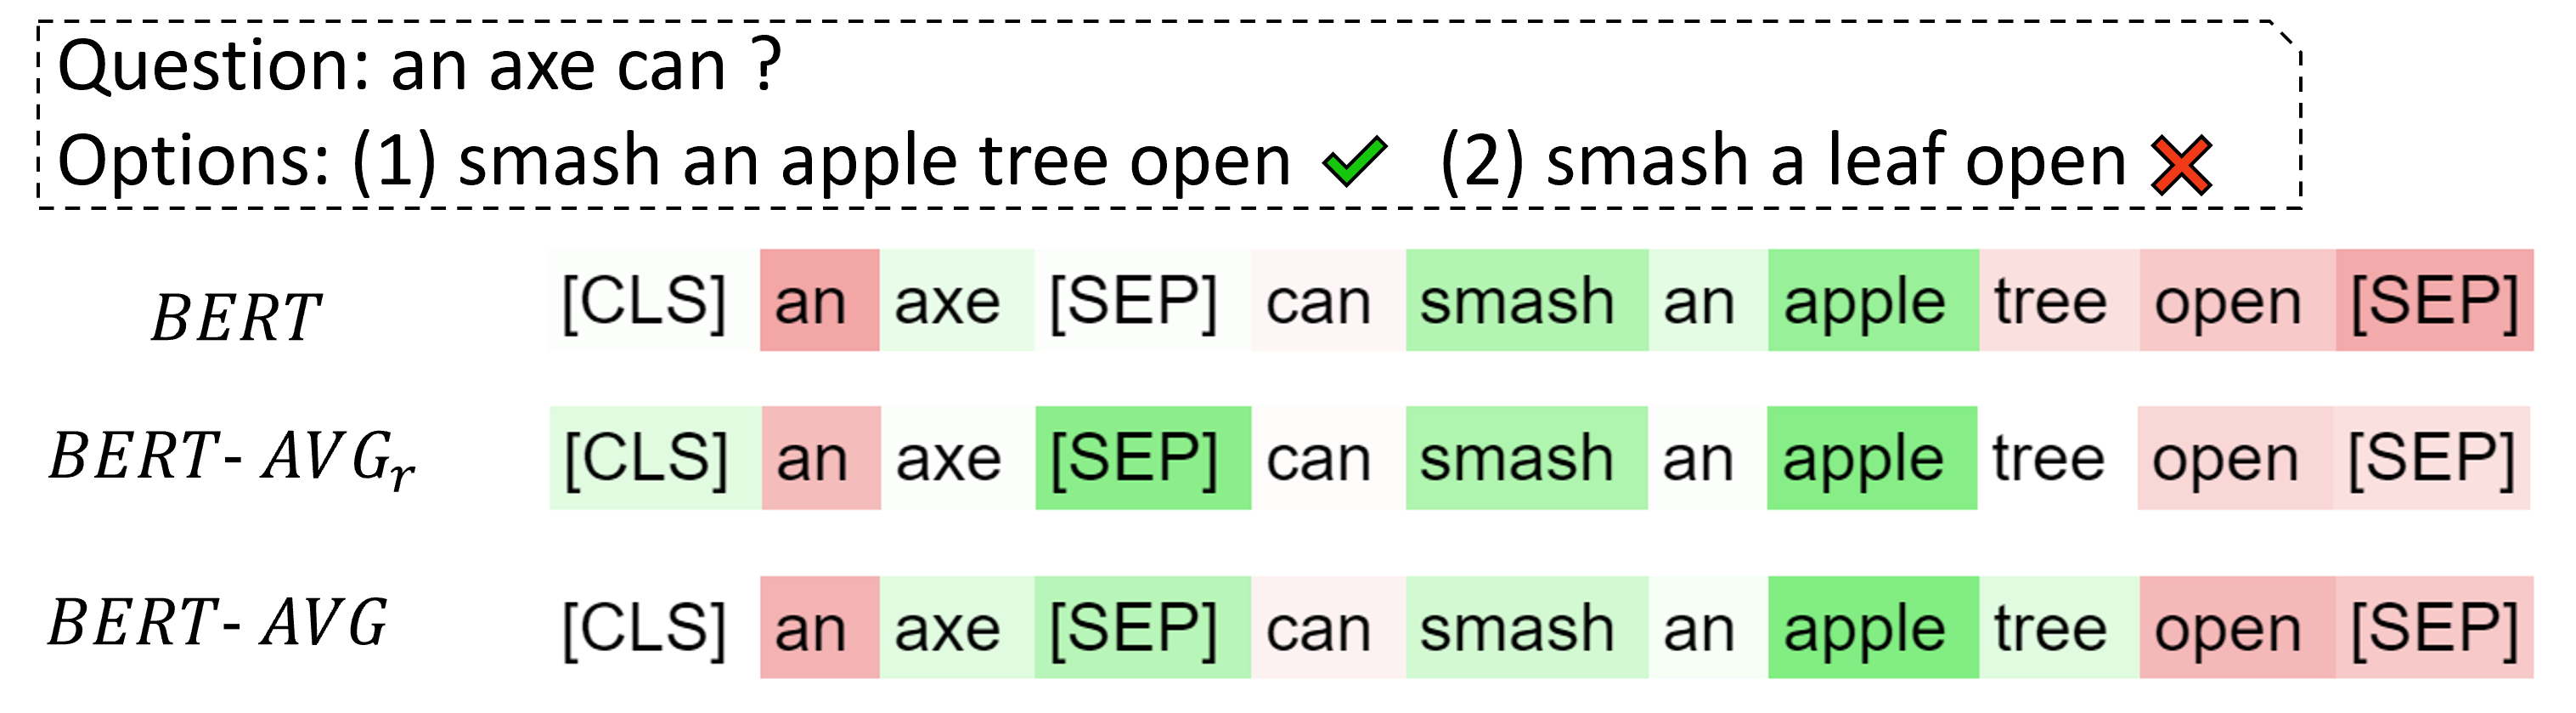
\includegraphics[width=1.0\columnwidth]{figures/IG.png}}
	\caption{Visualization using Integrated Gradient. Green/Red indicates positive/negative contribution.} \label{fig:IG}
\end{figure} 
